%
% METU Institute of Natural and Applied Sciences Thesis example 
%
% Edited and Commented by Utku Erdoğdu 2013, and a little touch by Irem Gokce Yildirim on Selma Suloglu's template
%
% Please read the explanations so that you can customize the document		
%
% Files needed by this document:
% metu.cls 
% metu11.def (if you will use 11pt fonts) 
% metu12.def (if you will use 12pt fonts)
% metu10.def (if you will use 10pt fonts)
%
% Possible Options Here:
%
% oneandhalf, double, single : Line spacing used in the thesis. Default and institute preference is
% single.
%
% 10pt, 11pt, 12pt : Font size Default is 10pt, which is institue choice. 
% 
% pntr, pntc, pnbt : Page number position. Options are top center, top right or bottom. Default and
% institute preference is page numbers at bottom. When page numbers are at the top bottom margins
% are skewed.
% 
% chaproman, chaparabic: Chapter numbering format. Options are roman numbers and arabic numbers.
% Default is roman, institute prefers arabic
%
% oneside, twoside : Printing style. Default is twoside, which is institute choice. In this style
% chapters begin from odd numbered pages.
%
% tr, eng : Document language. This is useful if you want to translate your thesis into
% Turkish. Then you give the option tr and use \ifturkish. . .\else. . .\fi  whenever you want 
% to do something only for Turkish or only for English. Default is eng. 
% IMPORTANT!! : For official institute documents you should not use this option. 
% The Turkish format is only supplied for custom translations.
%
% ceng,aee,arme.. : You can use the abbreviated form of your department here and there is no further need to
% define the department name below. If your department name is not among the below list of defined
% departments, you should use \department and \turkishdepartment macros to define the name of your
% department.
%
% Defined Departments and Abbreviations:
% --------------------------------------
% Computer Engineering : ceng
% Aerospace Engineering : aee
% Archaeometry : arme
% Architecture : arch
% Biochemistry : bch
% Biology : biol
% Biomedical Engineering : bme
% Biotechnology : btec
% Building Science : bs
% Cement Engineering : ceme
% Chemical Engineering : che
% Chemistry : chem
% City and Regional Planning : crp
% City Planning : cp
% Civil Engineering : ce
% Computational Design and Fabrication Technologies in Architecture : arcd
% Computer Education and Instructional Technology : cte
% Design Research for Interaction : iddi
% Earthquake Studies : eqs
% Earth System Science : ess
% Electrical and Electronics Engineering : ee
% Engineering Management : em
% Engineering Sciences : es
% Environmental Engineering : enve
% Food Engineering : fde
% Geodetics - Geographical Information Technologies : ggit
% Geological Engineering : geoe
% Hydrosystems Engineering : he
% Industrial Design : id
% Industrial Engineering : ie
% Mathematics : math
% Mechanical Engineering : mech
% Metallurgical and Materials Engineering : mete
% Micro and Nanotechnology : mnt
% Mining Engineering : mine
% Operational Research : or
% Petroleum and Natural Gas Engineering : pete
% Physics : phys
% Polymer Science and Technology : pst
% Regional Planning : rp
% Restoration : rest
% Secondary Science and Mathematics Education : ssme
% Software Engineering : se
% Statistics : stat
% Structural Mechanics : st
% 
% phd, ms : Degree Received. Ph.D. or M.S. Default is M.S.
%
% End of Options
\documentclass[a4paper,chaparabic,gate,ms,12pt,single]{metu}
% You can delete next line If your thesis does not have an appendix
\usepackage{appendix}
% Use your latex packages here

%\usepackage[a4paper]{geometry}
\usepackage{amsmath, amssymb}
\usepackage{enumitem}
\usepackage{caption}
\usepackage{tabularx}
\usepackage{multirow}
%

% End of Latex Packages
%
% Any personal Latex definition, decleration, etc.


% End of personal stuff
%
% Personal Information 
% ----------------------------
%
% Please check this part and fill in information about your thesis
%
% Name and Surname
\author{Your Name and Surname}
% Thesis Title English and Turkish
\title{Title}
\turkishtitle{Turkish Title}
% Department : English and Turkish
%
% Some of the departments are pre-defined, you need not redeclare them. You can use them by just
% giving an option to \documentclass. See documentation for options above. If you will define your 
% department here do not use ``Department'' or ``Bölümü'' words.
%\department{Computer Engineering}
%\turkishdepartment{Bilgisayar Mühendisliği}
%
%
% Date : You should indicate the month of your thesis defence in English.
% Default is this month
%
\date{Month Year}
%
% Approval Page Details
% --------------------------
% For each command you can give the title as optional parameter enclosed in [ ]
% This also handles the Turkish titles if you're planning to produce Turkish version of the
% document. If you'll hard code the title, you need to use turkish version of each command after
% the command itself
% 
% prof : Prof. Dr.
% assocprof : Assoc. Prof. Dr.
% assistprof : Assist. Prof. Dr.
% dr : Dr.
%
% Director of Institute
\director[prof]{Nazife Baykal}
% Head of Department
\headofdept[assocprof]{Hüseyin Hacıhabiboğlu}
%
% Supervisor : English and Turkish
\supervisor[assocprof]{Supervisor}
\cosupervisor[assocprof]{Co-Supervisor}
% \turkishsupervisor{  } %if you will hard-code the academic title
%
% Affiliation of Supervisor in English and possibly in Turkish
\departmentofsupervisor{Department of Supervisor, METU}
% Co Supervisor if Any : English and Turkish
% You can just delete the next line if you don't have a co-supervisor
%\cosupervisor[assocprof]{Bedir Tekinerdoğan}
% \turkishcosupervisor{Prof. Dr. Reda Alhajj} %if you will hard-code the academic title
% Affiliation of Co-Supervisor
% You can just delete the next line if you don't have a co-supervisor
\departmentofcosupervisor{Department of Coadvisor, METU}
%
% Committee Members
% In general members are sorted according to their academic titles
%
% Proffesors (1)
% Associate Professors (2)
% Assistant Professors (3)
% Other (4)
% 
% IMPORTANT:  All affiliatons should fit in a single line
% If affiliation line is broken into two lines you should shorten the affiliation by using 
% abbrevations or any other means
%
% First committee member should be the chair of examining committee
% Typically the chair is one of the highest ranked committee members
% Ask your supervisor if you are not sure
\committeememberi[prof]{Committee Member Name and Surname}
\affiliationi{Dept of Committee Member, METU}
% Second committee member is always your supervisor
\committeememberii[assocprof]{Committee Member Name and Surname}
\affiliationii{Dept of Committee Member, METU}
% If you are an M.Sc. student and your Co-Supervisor is in your 
% examination committee, then third committee member is always your co-supervisor
%
% IMPORTANT: If you are Ph.D. student your co-supervisor can not be in your 
% examination committee.
\committeememberiii[assocprof]{Committee Member Name and Surname}
\affiliationiii{Dept of Committee Member, METU}
% Fourth committee member
\committeememberiv[assistprof]{Committee Member Name and Surname}
\affiliationiv{Dept of Committee Member, METU}
% Fifth committee member
\committeememberv[assistprof]{Committee Member Name and Surname}
\affiliationv{Dept of Committee Member, Çankaya University}
%
% Keywords : English & Turkish, Comma seperated
\keywords{keyword1,keyword2,keyword3,keyword4,keyword5}
\anahtarklm{kelime1,kelime2,kelime3,kelime4,kelime5}
%
% Abstract in English
%
\abstract{Abstract in English}
%
% Turkish Abstract
%
\oz{Abstract in Turkish} 
%
% Dedication 
\dedication{\textit{Dedication}}
%
%
% Acknowledgements   
\acknowledgments{
Acknowledgements
}
%
% End of Personal and Introductory Information
%%%%%%%%%%%%%%%%%%%%%%%%%%%%%%%%%5

%%% !!! This two should be last lines before \begin{document}, do no move them !!!
\usepackage[pdftex]{hyperref}
\usepackage[all]{hypcap}
\usepackage{todonotes}
\usepackage{graphicx}
\graphicspath{ {./images/} }
\usepackage{rotating}
\usepackage{xy} 
\usepackage{booktabs}
\usepackage{pifont}
\usepackage{color}
\usepackage{listings}
\usepackage{pdfpages}
\usepackage{array}
\newcolumntype{M}{>{\centering\arraybackslash}m{\dimexpr.25\linewidth-2\tabcolsep}}
\renewcommand\lstlistingname{XChor Language - }
\def\lstlistingautorefname{XChorCode.}
\lstset{
language = java,
basicstyle=\small,
numbers=left,
numbersep=10pt,
numberstyle=\tiny\color{black},
stepnumber=1,
tabsize=2,
showspaces=false, 
frame=single,
breaklines=true,
escapeinside=~~
}
\usepackage{float}
\restylefloat{figure}
\newcommand{\tab}{\hspace*{2em}}
\DeclareGraphicsExtensions{.pdf,.png,.jpg}

\begin{document}
% Preliminaries
\begin{preliminaries}
% If you are willing to use any custom stuff before Chapters, put it here
% Such as List of Abbreviations
% Check the abbreviations.tex for a template list of abbreviations

\begin{theglossary}{LONGESTABBRV}

\item[3D] Three Dimensional
\item[NPC] Non-Player Character
\item[MDA] Mechanics, Dynamics, Aesthetics (Framework)
\item[MMO] Massively Multiplayer Online Game
\item[PENS] Player Experience of Need Satisfaction
\item[RPG] Role Playing Game
\item[SDT] Self-Determination Theory

\end{theglossary}

% End of Preliminaries
\end{preliminaries}
%   
% Latex content Goes Here 
% 
%
% CHAPTER 1
\chapter {INTRODUCTION}
\label {chp:introduction}
Introduction here.

In this study, the following hypotheses are proposed (See Figure~\ref{fig:framework}).

\begin{itemize}
\item \textbf {H1 :} Example hypothesis.
\end{itemize}

\begin{figure}[h]
\centering
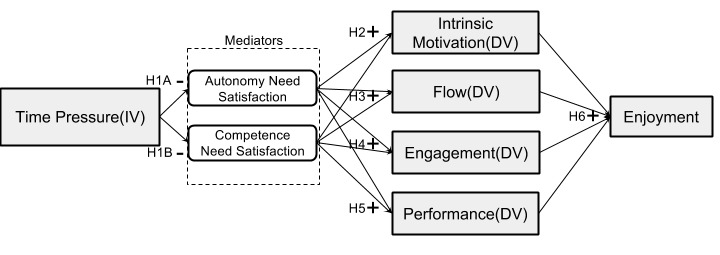
\includegraphics [width=1\textwidth,clip]{images/Figure_1_Framework}
\caption[CaptionforListofFigures]{Caption}
\label {fig:framework}
\end{figure}

Outline of the thesis is as follows:
\begin{itemize}
\item Chapter 2 provides..
\item Chapter 3 introduces..
\item Chapter 4 includes ..
\item Chapter 5 presents ..
\end{itemize}
% CHAPTER 2
\chapter {RELATED WORK AND BACKGROUND}
\label {chp:relatedworks}

Contents here.

\section {Section1}
Example citation. \cite{RyanDeci2000bSDT}. 

\section {Section2}
Contents here \cite{RyanRigby2011glued, Baldwin2014DynamicDifficulty, NPD2014Report, Quick2013ModelingEnjoyment, Dennie2012AutonomyMotivation, Ryan2000Rewards, McNamara2010PointsFeedback, unityGame}.

\subsection {Subsection2.1}
\begin{description}
\item[Item1] \hfill \\
Contents here.

\item[Item2] \hfill \\
Contents here. 
\end{description}
% CHAPTER 3
\chapter {METHOD}
\label {chp:method}
Contents here.

\section {Participants}
Contents here.
\section {Measures}
Contents here.
		\subsubsection {Measure1}
Contents here. (See Appendix~\ref{chp:appendixB}).
		\subsubsection {Measure2}
Contents here. (See Appendix~\ref{chp:appendixC}). Cronbach's alpha\footnote{\label{fn}In statistics, Cronbach's alpha ($\alpha$) coefficient is used as an estimation of the reliability of a scale based on the correlation between the items of the scale} was .85.
		\subsubsection {Measure3}
		Contents here.\footnote{Retrieved from \scriptsize \url{http://www.selfdeterminationtheory.org/basic-psychological-needs-scale/}} by Deci et al.\cite{deci2001need} ``Some quotation''($\alpha = .84$)\footnotemark[\getrefnumber{fn}] (See Appendix~\ref{chp:appendixD}). 



% CHAPTER 4
\chapter {RESULTS}%and evaluation
\label {chp:results}
Contents here.

\section {Preliminary Analysis}
	\subsection {Manipulation Check}
Contents here.\\

\begin{table}[h]
\captionsetup{labelfont=bf, justification=justified,singlelinecheck=false}
\caption[CaptionforListofTables]{Caption}
\label {table:manipulationcheck}
\begin{tabularx}{1.0\textwidth}{lccl}
\hline
\multicolumn{1}{c}{} & \begin{tabular}[c]{@{}c@{}}Control Group \\ ($n$=50)\end{tabular} & \begin{tabular}[c]{@{}c@{}}Experimental Group\\ ($n$=51)\end{tabular} &  \\ \hline
\multicolumn{1}{c}{Scale Name} & \multicolumn{2}{c}{$M$ ($SD$)} & $t$(99) \\ \hline
IV & 2.64 (2.02) & 5.45 (1.72) & 7.53$^{\ast}$ \\
IV & 2.29 (1.62) & 4.39 (2.07) & 5.65$^{\ast\ast\ast}$ \\
IV & 2.30 (1.61) & 2.96 (1.95) & 1.86 \\ \hline
$^{\ast}p$ \textless .05, $^{\ast\ast\ast}p$ \textless .001 & \multicolumn{1}{l}{} & \multicolumn{1}{l}{} & \multicolumn{1}{l}{}
\end{tabularx}
\end{table}

\section {Primary Analysis}
Contents here. It was revealed that the players who were subjected to time pressure ($M = 5.38, SD = 1.02$) experienced more flow than the participants in the control group who were not ($M = 4.84, SD = 1.44$); $t(99) = 2.21, p = .030$ (See Table~\ref{table:primaryresults}). 

\begin{table}[h]
\captionsetup{labelfont=bf, justification=justified,singlelinecheck=false}
\caption[CaptionforListofTables]{Caption}
\label {table:primaryresults}
\begin{tabularx}{1.0\textwidth}{lccl}
\hline
\multicolumn{1}{c}{} & \begin{tabular}[c]{@{}c@{}}Control Group \\ ($n$=50)\end{tabular} & \begin{tabular}[c]{@{}c@{}}Experimental Group\\ ($n$=51)\end{tabular} &   \\ \hline
\multicolumn{1}{c}{Dependent variables} & \multicolumn{2}{c}{$M$ ($SD$)} & $t$ (99) \\ \hline
DV & 3.03 (1.31) & 3.37 (1.36) & 1.24 \\
DV & 4.83 (1.56) & 4.86 (1.40) & 0.11\\
DV & 3.82 (0.88) & 3.96 (0.90) & 0.76 \\
DV & 4.84 (1.44) & 5.38 (1.02) & 2.21$^{\ast}$ \\
DV & 3.52 (0.88) & 3.81 (0.95) & 1.62 \\
DV & 92.7 (17.4) & 94.5 (11.3) & 0.62 \\
DV & 4.83 (1.41) & 4.94 (1.01) & 0.46 \\
DV & 130.62 (39.4) & 110.49 (10.9) & 3.51$^{\ast\ast}$ \\ \hline
$^{\ast}p$ \textless .05, $^{\ast\ast}p$ \textless .01 & \multicolumn{1}{l}{} & \multicolumn{1}{l}{} & \multicolumn{1}{l}{}
\end{tabularx}
\end{table} 

Contents here. (See Table~\ref{table:gameendconditions}).

\begin{table}[H]
\captionsetup{labelfont=bf, justification=justified,singlelinecheck=false}
\caption[CaptionforListofTables]{Caption}
\label {table:gameendconditions}
\begin{tabular}{lcc}
\hline
\multicolumn{1}{c}{} & \begin{tabular}[c]{@{}c@{}}Control Group \\ ($n$=53)\end{tabular} & \begin{tabular}[c]{@{}c@{}}Experimental Group \\ ($n$=53)\end{tabular} \\ \hline
\multicolumn{1}{c}{Subgroups} & \multicolumn{2}{c}{$n$} \\ \hline
Subgroup & 50 & 29 \\
Subgroup  & 3 & 2 \\
Subgroup & - & 22 \\ \hline
\end{tabular}
\end{table}


One-Way between subjects ANOVA. However, there was a significant difference in perceived time pressure, flow and engagement at the $p<.05$ level for three conditions [$F(2,98) = 21.4, p < .001$ and $F(2,98) = 3.70, p = .028$ and $F(2,98) = 3.24, p = .043$ respectively] (See Table~\ref{table:anovaresults}).

\begin{table}[h]
\captionsetup{labelfont=bf, justification=justified,singlelinecheck=false}
\caption[CaptionforListofTables]{Caption}
\label {table:anovaresults}
\resizebox{\columnwidth}{!}{
\begin{tabular}{lcccccl}
\hline
 & \begin{tabular}[c]{@{}c@{}}Control Group \\ ($n$ = 53)\end{tabular} &  & \multicolumn{2}{c}{\begin{tabular}[c]{@{}c@{}}Experimental Group \\ ($n$ = 53)\end{tabular}} & \multicolumn{1}{l}{} & \multicolumn{1}{l}{} \\ \cline{2-2} \cline{4-5}
 & \begin{tabular}[c]{@{}c@{}}Successful \\ ($n$ = 50)\end{tabular} &  & \begin{tabular}[c]{@{}c@{}}Successful \\ ($n$ = 29)\end{tabular} & \begin{tabular}[c]{@{}c@{}}No Time \\ ($n$ = 22)\end{tabular} & \multicolumn{1}{l}{} & \multicolumn{1}{l}{} \\ \cline{2-5}
\multicolumn{1}{c}{} & \multicolumn{4}{c}{$M$} & $F$ (2,98) & Sig. \\ \hline
IV & 2.29 &  & 3.76 & 5.23 & 21.4 & .000$^{\ast\ast\ast}$ \\
DV & 3.03 &  & 3.20 & 3.56 & 1.23 & .30 \\
DV & 4.83 &  & 5.23 & 4.38 & 2.16 & .12 \\
DV & 3.82 &  & 3.83 & 4.12 & 0.96 & .39 \\
DV & 4.84 &  & 5.14 & 5.69 & 3.70 & .028$^{\ast}$ \\
DV & 3.52 &  & 3.60 & 4.10 & 3.24 & .043$^{\ast}$ \\
DV & 92.7 &  & 98.1 & 89.8 & 2.31 & .11 \\ 
DV & 4.83 &  & 4.93 & 4.97 & .11 & .89 \\ \hline
$^{\ast}p$ \textless .05, $^{\ast\ast\ast}p$\textless .001 & \multicolumn{1}{l}{} & \multicolumn{1}{l}{} & \multicolumn{1}{l}{} & \multicolumn{1}{l}{} & \multicolumn{1}{l}{} & \multicolumn{1}{l}{}
\end{tabular}}
\end{table}

Post Hoc comparisons using the Tukey HSD test indicated that the mean scores of perceived time pressure for successful subgroup of control group ($M = 2.29, SD = 1.62$) were significantly lower from successful ($M = 3,76, SD = 2.08$) and no time subgroups of experimental group ($M = 5.23, SD = 1.77$). (See Figure~\ref{fig:means}).

\begin{figure}[h]
\centering
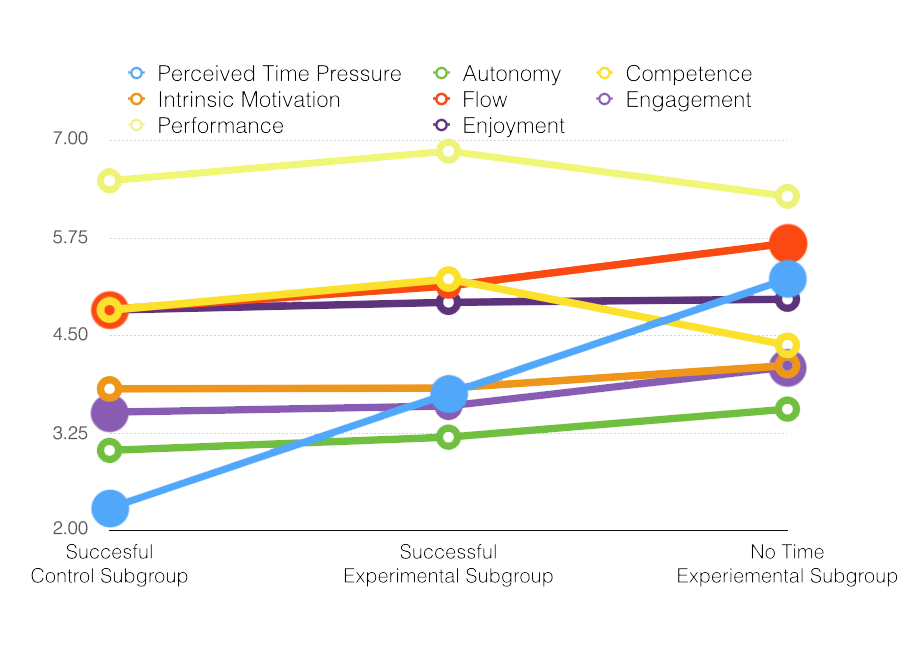
\includegraphics [width=.9\textwidth,clip]{images/Figure_6_Results}
\caption[CaptionforListofFigures]{Caption. \it {Note: Some note.}}
\label {fig:means}
\end{figure}

Although there was no significant difference in competence between both two main groups (control and experimental) and three subgroups, it approached significance between successful and no time subgroups of experimental group ($M = 5.23, SD = 1.22$ and $M = 4.38, SD = 1.48$ with $p = .10$, respectively). Furthermore, positive correlation between competence and performance [$r$ = .43, $n$ = 53, $p$ = .001] was revealed in the results of experimental group (See Table~\ref{table:correlationBygroup}).  

\begin{figure}[h]
\centering
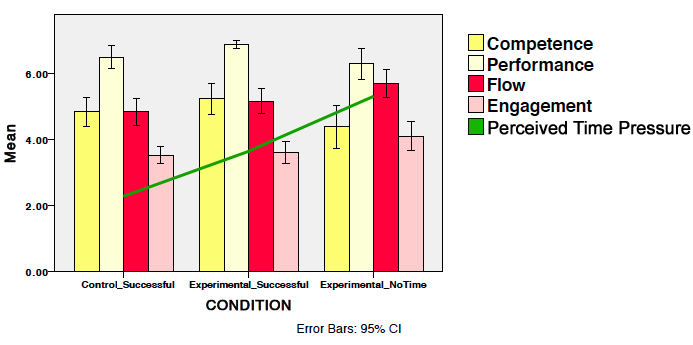
\includegraphics [width=1\textwidth,clip]{images/Figure_7_Discussion}
\caption[CaptionforListofFigures]{Caption}
\label {fig:subgroups}
\end{figure}

\begin{table}[h]
\captionsetup{labelfont=bf, justification=justified,singlelinecheck=false}
\caption[CaptionforListofTables]{Caption}
\label {table:correlationBygroup}
\resizebox{\columnwidth}{!}{
\begin{tabular}{llllllllll}
\hline
 &  & \multicolumn{8}{c}{Control Group} \\ \cline{3-10} 
 &  & IV & DV & DV & \begin{tabular}[c]{@{}l@{}}Long \\ DV\end{tabular} & DV & DV & DV & DV \\ \cline{2-10} 
\multicolumn{1}{l|}{\multirow{8}{*}{\begin{sideways}Experimental Group\end{sideways}}} & IV & - & .31$^{\ast}$ & -.16 & .48$^{\ast\ast}$ & .21 & .30$^{\ast}$ & -.04 & .06 \\
\multicolumn{1}{l|}{} & DV & .17 & - & .32$^{\ast}$ & .53$^{\ast\ast}$ & .05 & .25 & .01 & .46$^{\ast\ast}$ \\
\multicolumn{1}{l|}{} & DV & -.13 & .33$^{\ast}$ & - & .26 & .33$^{\ast}$ & .34$^{\ast}$ & .26 & .56$^{\ast\ast}$ \\
\multicolumn{1}{l|}{} & Long DV & .43$^{\ast\ast}$ & .41$^{\ast\ast}$ & .09 & - & .54$^{\ast\ast}$ & .61$^{\ast\ast}$ & -.10 & .77$^{\ast\ast}$ \\
\multicolumn{1}{l|}{} & DV & .12 & .44$^{\ast\ast}$ & .14 & .38$^{\ast\ast}$ & - & .65$^{\ast\ast}$ & .10 & .42$^{\ast\ast}$ \\
\multicolumn{1}{l|}{} & DV & .27 & .63$^{\ast\ast}$ & .15 & .61$^{\ast\ast}$ & .67$^{\ast\ast}$ & - & .06 & .46$^{\ast\ast}$ \\
\multicolumn{1}{l|}{} & DV & .08 & -.10 & .43$^{\ast\ast}$ & -.11 & -.30$^{\ast}$ & -.23 & - & -.07 \\
\multicolumn{1}{l|}{} & DV & .14 & .41$^{\ast\ast}$ & .35$^{\ast\ast}$ & .66$^{\ast\ast}$ & .31$^{\ast}$ & .38$^{\ast\ast}$ & -.04 & - \\ \cline{2-10} 
 & $^{\ast}p$ \textless .05, $^{\ast\ast}p$\textless .01 &  &  &  &  &  &  &  & \\ 
 & \multicolumn{9}{l}{\textit{Note.} $n$ = 53 \textit{for both groups. Correlations for Experimental Group lies on the lower part of the diagonal, correlations for Control}} \\ 
 & \multicolumn{9}{l}{\textit{Group lies on the upper part of the diagonal.}}
\end{tabular}}
\end{table}


\begin{table}[H]
\captionsetup{labelfont=bf, justification=justified,singlelinecheck=false}
\caption[CaptionforListofTables]{Caption}
\label {table:correlation}
\resizebox{\columnwidth}{!}{
\begin{tabular}{lllllllll}
\hline
 & \begin{tabular}[c]{@{}l@{}}Long \\ IV\end{tabular} & DV & DV & \begin{tabular}[c]{@{}l@{}}Long \\ DV\end{tabular} & DV & DV & DV & DV \\ \hline
Long IV & - &  &  &  &  &  &  &  \\
DV & .27$^{\ast\ast}$ & - &  &  &  &  &  &  \\
DV & -.13 & .32$^{\ast\ast}$ & - &  &  &  &  &  \\
Long DV & .44$^{\ast\ast}$ & .48$^{\ast\ast}$ & .18 & - &  &  &  &  \\
DV & .25$^{\ast}$ & .24$^{\ast}$ & .26$^{\ast\ast}$ & .48$^{\ast\ast}$ & - &  &  &  \\
DV & .33$^{\ast\ast}$ & .46$^{\ast\ast}$ & .24$^{\ast}$ & .62$^{\ast\ast}$ & .65$^{\ast\ast}$ & - &  &  \\
DV & .05 & -.03 & .33$^{\ast\ast}$ & -.09 & -.02 & -.06 & - &  \\
DV & .11 & .43$^{\ast\ast}$ & .48$^{\ast\ast}$ & .72$^{\ast\ast}$ & .39$^{\ast\ast}$ & .42$^{\ast\ast}$ & -.06 & - \\ \hline
\textit{Note.} $n$ = 106. &  &  &  &  &  &  &  & \\
 \multicolumn{9}{l}{$^{\ast}p$ \textless .05, $^{\ast\ast}p$\textless .01}
\end{tabular}}
\end{table}

\section {Discussion}
Contents here. (See Table~\ref{table:anovaresults}).  (See Figure~\ref{fig:means}).


% CHAPTER 5
\chapter {CONCLUSION AND FUTURE WORK}
\label {chp:conclusion}
Contents here.
\section {General Limitations}
	\subsection {Participants}
	Contents here. 
	
	\subsection {Other Limitations}
	Contents here.  
		
\section {Implications and Future Works}
Contents here.

\section {Conclusion}
Contents here.






%just change it here if you want acm style etc.
\bibliographystyle{ieeetr}	
%
% References in Bibtex format goes into below indicated file with .bib extension
\bibliography{thesis_references}
% You can use full name of authors, however most likely some of the Bibtex entries you will find, will use abbreviated first names
% If you don't want to correct each of them by hand, you can use abbreviated style for all of the references

\appendix
\chapter {Informed Consent Form}
\label {chp:appendixA}

\section* {Genel Bilgiler}
Bu çalışma ODTÜ Enformatik Enstitüsü Oyun Teknolojileri Yüksek Lisans Programı öğrencilerinden İrem Gökçe Yıldırım tarafından yürütülmektedir. Bu form sizi araştırma koşulları hakkında bilgilendirmek icin hazırlanmıştır.

Bu calışmanın amacı bazı oyun tasarım özellikleri ve edinilen psikolojik deneyimlerin arasindaki ilişkileri incelemektir. Arastırma internet üzerinden doldurulacak bir anket, devamında tamamlanacak olan bir laboratuvar çalışmasını içermektedir. Anket yaklaşık 5 dakika, laboratuvar çalışması ise 15 dakika sürecektir.

Araştırmada yaklaşık 100 katılımcı hedeflenmektedir. Üniversite öğrencileri katılımcı olarak davet edilecek, çalışmaya katılanlar bu duyurunun yapildiği ders için bonus puan alacaklardir. Alinacak puan dersin oğretim üyesi tarafından belirlenecektir.
\section* {Riskler ve Faydalar}
Araştırma katılımcı için herhangi bir risk veya fayda içermemektedir.
\section* {Gönüllülük Esası}
Bu çalışmaya katılmak tamamen gönüllülük esasına dayalıdır. Çalışmayı istediginiz zaman bırakabilir, çalışma esnasında cevap vermek istemediğiniz sorular olursa boş bırakabilirsiniz.
\section* {Gizlilik Esası}
Çalismaya katılanlardan toplanan veriler tamamen gizli tutulacak, veriler ve kimlik bilgileri herhangi bir şekilde eşleştirilmeyecektir. Katılımcıların isimleri bağımsız bir listede toplanacaktır. Ayrıca toplanan verilere sadece araştırmacılar ulaşabilecektir. Bu araştırmanın sonuçları bilimsel ve profesyonel yayınlarda veya eğitim amaçlı kullanılabilir, fakat katılımcılarin kimliği gizli tutulacaktır.
\section* {Irtibat}
Çalışmayla ilgili soru ve yorumlarınızı araştırmacıya gokce.aydin@metu.edu.tr adresinden iletebilirsiniz veya ..`'lu telefondan İrem Gökçe Yıldırım`'a ulaşabilirsiniz.
\section* {Katılımcı Onayı}
\textbf{Yukarıdaki bilgileri okudum ve bu araştırmaya gönüllü olarak katiımayı kabul ediyorum.}
\vskip1.5cm plus0pt minus2mm \nointerlineskip
\vbox{
\parbox[b]{7cm}{\begin{center}
{\mbox{\textbf{Ad-Soyad:}}}
\end{center}\nointerlineskip}
\parbox[b]{7cm}{\begin{center}
{\mbox{\textbf{Imza}}}
\end{center}}}

\chapter {Demographics and Game Play Questionnaire}
\label {chp:appendixB}

\begin{enumerate}
\item Yaşınız?\\
	\rule{5cm}{1pt}
\item Cinsiyetiniz?\\
	\begin{math}
	\square \mbox{ Kadın} \\
	\square \mbox{ Erkek}
	\end{math}
\item Lisans Anadalı Fakülteniz?\\
	\begin{math}
	\bigcirc \mbox{ Mühendislik}\\
	\bigcirc \mbox{ Fen Bilimleri}\\
	\bigcirc \mbox{ Mimarlık}\\
	\bigcirc \mbox{ Eğitim}\\
	\bigcirc \mbox{ Sosyal Bilimler}\\
	\bigcirc \mbox{ İktisadi ve İdari Bilimler}\\
	\bigcirc \mbox{ Diğer (Lütfen Belirtiniz) }\rule{5cm}{1pt}
	\end{math}
\item Video oyunları oynar mısınız?\\
	\begin{math}
	\square \mbox{ Evet} \\
	\square \mbox{ Hayır}
	\end{math}
\item *Haftada kaç saat video oyunları oynarsınız?\\
	\begin{math}
	\bigcirc \mbox{ 1 saatten az}\\
	\bigcirc \mbox{ 1-5}\\
	\bigcirc \mbox{ 5-10}\\
	\bigcirc \mbox{ 10-15}\\
	\bigcirc \mbox{ 15'den fazla}\\
	\end{math}
\item *Kaç senedir video oyunları oynuyorsunuz?\\
	\begin{math}
	\bigcirc \mbox{ 1'den az}\\
	\bigcirc \mbox{ 1-3}\\
	\bigcirc \mbox{ 3-5}\\
	\bigcirc \mbox{ 5-7}\\
	\bigcirc \mbox{ 7'den fazla}\\
	\end{math}
\item Hangi tip oyunları oynamaktan hoslanırsınız?(Çoklu seçim yapabilirsiniz.)\\
	\begin{math}
	\square \mbox{ Birinci Şahis Nişancı Oyunları (First Person Shooter)}\\
	\square \mbox{ Rol Yapma Oyunları (Role Playing Games)}\\
	\square \mbox{ Devasa Çok Oyunculu Çevrimici Rol Yapma Oyunları (MMORPG)}\\
	\square \mbox{ Aksiyon Oyunları (Action Games)}\\
	\square \mbox{ Macera Oyunları (Adventure Games)}\\
	\square \mbox{ Puzzle Oyunları (Puzzle Games)}\\
	\square \mbox{ Strateji Oyunları}\\
	\square \mbox{ Gerçek Zamanlı Strateji Oyunları (Real Time Strategy Games)}\\
	\square \mbox{ Sıra Tabanlı Strateji Oyunları (Turn Based Strategy Games)}\\
	\square \mbox{ Gündelik Oyunlar (Casual Games)}\\
	\square \mbox{ Platform Oyunları}\\
	\square \mbox{ Spor Oyunları}\\
	\square \mbox{ Simulasyonlar}\\
	\square \mbox{ Diğer(Lütfen Belirtiniz) }\rule{5cm}{1pt}
	\end{math}
\item Oyunlarda en çok hoşunuza giden özellikler nelerdir?(Çoklu seçim yapabilirsiniz.)\\
	\begin{math}
	\square \mbox{ Arayüz}\\
	\square \mbox{ Karakterler-Modeller}\\
	\square \mbox{ Ses Efektleri-Müzik}\\
	\square \mbox{ Stratejik Davranabilme}\\
	\square \mbox{ Zaman Baskısı}\\
	\square \mbox{ Oyun Mekaniği}\\
	\square \mbox{ Hareket Kabiliyetleri ve Kontroller}\\
	\square \mbox{ Çoklu Oyun Oynayabilme}\\
	\square \mbox{ Hikaye}\\
	\square \mbox{ Başarı ve Kazanımlar}\\
	\square \mbox{ Avatar Özelleştirebilme}\\
	\square \mbox{ Diğer(Lütfen Belirtiniz) }\rule{5cm}{1pt}
	\end{math}
\item Kullandıgınız oyun platformları nelerdir?(Çoklu seçim yapabilirsiniz.)\\
	\begin{math}
	\square \mbox{ PC}\\
	\square \mbox{ Xbox}\\
	\square \mbox{ PlayStation}\\
	\square \mbox{ PlayStation Portable}\\
	\square \mbox{ Wii}\\
	\square \mbox{ Android Mobil Cihazlar}\\
	\square \mbox{ iOS Mobil Cihazlar}\\
	\square \mbox{ Diğer(Lütfen Belirtiniz) }\rule{5cm}{1pt}
	\end{math}
\item Kendinizi nasıl hedefi olan bir oyuncu olarak tanımlarsınız?\\
	\begin{math}
	\bigcirc \mbox{ Öğrenmeye ve yetkinliklerini arttırmaya çalışan}\\
	\bigcirc \mbox{ Öğrenememekten ve yetkinliklerini arttıramamaktan endişe duyan}\\
	\bigcirc \mbox{ Diğerlerinden daha iyi performans göstermeye çalışan}\\
	\bigcirc \mbox{ Diğerlerinden kötü perfomans göstermekten kaçınan}
	\end{math}
\end{enumerate}


\chapter {Exemplary Scale}
\label {chp:appendixC}
Aşağıdaki her bir ifadenin sizin düşüncenize göre ne kadar doğru olduğunu, aşağıdaki ölçek skalasını kullanarak belirtiniz.\\

\hspace{2.5cm}\makebox[10cm][s]{1 2 3 4 5 6 7} \par
\hspace{1cm}\makebox[13cm][s]{\parbox[c]{3cm}{\centering Kesinlikle katılmıyorum} \parbox{2.7cm}{\centering Ne katılıyorum ne katılmıyorum} \parbox{3cm}{\centering Kesinlikle katılıyorum}} \\

\begin{enumerate}
\item Statement Content.
\item Statement Content.
\item Statement Content.
\item Statement Content.
\end{enumerate}


\chapter {Exemplary Scale}
\label {chp:appendixD}
Aşağıdaki her bir ifadenin sizin düşüncenize göre ne kadar doğru olduğunu, aşağıdaki ölçek skalasını kullanarak belirtiniz.\\

\hspace{2.5cm}\makebox[10cm][s]{1 2 3 4 5 6 7} \par
\hspace{1cm}\makebox[13cm][s]{\parbox[c]{3cm}{\centering Kesinlikle katılmıyorum} \parbox{2.7cm}{\centering Ne katılıyorum ne katılmıyorum} \parbox{3cm}{\centering Kesinlikle katılıyorum}} \\


\section*{Sub Scale}
\begin{enumerate}
\item Statement Content.
\item Statement Content.
\item Statement Content.
\end{enumerate}

\section*{Sub Scale}
\begin{enumerate}
\item  Statement Content.
\item  Statement Content.
\item  Statement Content.
\end{enumerate}


\chapter {Exemplary Scale}
\label {chp:appendixE}

The following player data is collected during game play:
\begin{enumerate}[label=\textbf{\arabic*}]
\item \textbf{Item1:} Contents here.
 \begin{enumerate}
 	\item Data1: Contents here.
 	\item Data2: Contents here.
 	\item Data3:Contents here.
 \end{enumerate}
\item \textbf{Item2:} Contents here.
\end{enumerate}



\end{document}